\section{Introduction}\label{sec:intro}
Text-based program editors are flexible and expressive user interfaces
so it is little wonder that they remain dominant decades after the teletype.
However, textual user interfaces are not the best tool for every computational job.
% In particular, there are countless 
% data types for which a non-textual
% user interface may situationally be more appropriate.

As a simple example, consider a record type
classifying RGBA-encoded colors. 
It is possible to select a particular color by entering
an expression of this type in a text editor, e.g. \li{\{ r: 255, g: 178, b: 45, a: 100 \}}. 
The problem with this textual user interface for color selection is that 
it offers no live feedback about which color has been selected 
and limited editing affordances for tweaking the selected color.
Analagous critiques apply to strictly textual user interfaces for 
countless other data structures,
such as vector graphics,
animation parameters,
musical sequences,
audio filters,
board game states, 
GUI widgets and layouts,
tabular data, 
plots,
geospatial data, 
neural network diagrams, 
biological neuron models, 
mathematical diagrams, 
and so on.

% It is difficult for the programmer, or anyone subsequently reading or modifying the code, to know which color is represented
% and to interactively tweak that color.

Practitioners in domains where manipulating data of types like these is 
a central activity 
have largely eschewed general-purpose programming environments 
in favor of more specialized graphical end-user applications, like %
image and video editors, music composition software, level design tools, 
and bespoke GUIs written by students or lab technicians, 
in large part because these applications 
take seriously the need for domain-specific forms of live feedback, 
graphical data representations, and 
direct manipulation affordances, 
e.g. color palettes, visual timelines, interactive plots, and maps.

The tragedy is that these applications have 
limited support for abstraction and composition.
It is difficult, for example, to bind a
color to a variable for use in multiple locations in an
otherwise directly constructed game map,
or to define a function that computes portions of an 
otherwise directly constructed vector graphic,
or to transform a directly constructed musical sequence 
by passing it through a series of symbolically defined functions.
Moreover, it is difficult to add new affordances or to compose
affordances in ways that the application developer did not anticipate.
Users cannot easily make even simple changes like replacing a numeric text box in a dialog with a slider,
much less more ambitious changes like installing an alternative visual interface for expressing geospatial data queries 
into a database frontend.

% Better support for manipulating data of types like these would be particularly helpful for users engaging in
% live and exploratory programming in domains like web design, media production,
% and data analysis. Indeed, 

This paper aims to resolve this tension between
programmatic and direct manipulation user interfaces by designing 
a programming environment that
is able to surface GUIs when working with types for which
they are useful, while retaining full support for symbolic program manipulation
and the abstraction and composition mechanisms
available in modern general-purpose programming languages.

\subsection{Background}\label{sec:background}
\definecolor{mygray}{rgb}{0.93, 0.93, 0.93}
\definecolor{shadecolor}{named}{mygray}

\begin{figure*}
  \begin{minipage}[t]{0.38\textwidth}
    \begin{subfigure}[t]{\linewidth}
    \begin{snugshade}
      \vspace*{-2mm}
      \caption{\textbf{Prior Work:} Graphite}
      \vspace*{1mm}
     \end{snugshade}
      \vspace*{1.5mm}
      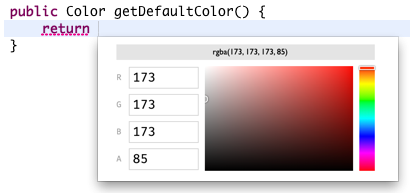
\includegraphics[width=\linewidth]{graphite-color-palette.png}
      \vspace*{2mm}
    \end{subfigure}
    
    \begin{subfigure}[t]{\linewidth}
     \begin{snugshade}
      \vspace*{-2mm}
      \caption{\textbf{This Paper:} Livelits are live and compositional}
      \vspace*{1mm}
     \end{snugshade}
      \vspace*{1.5mm}
      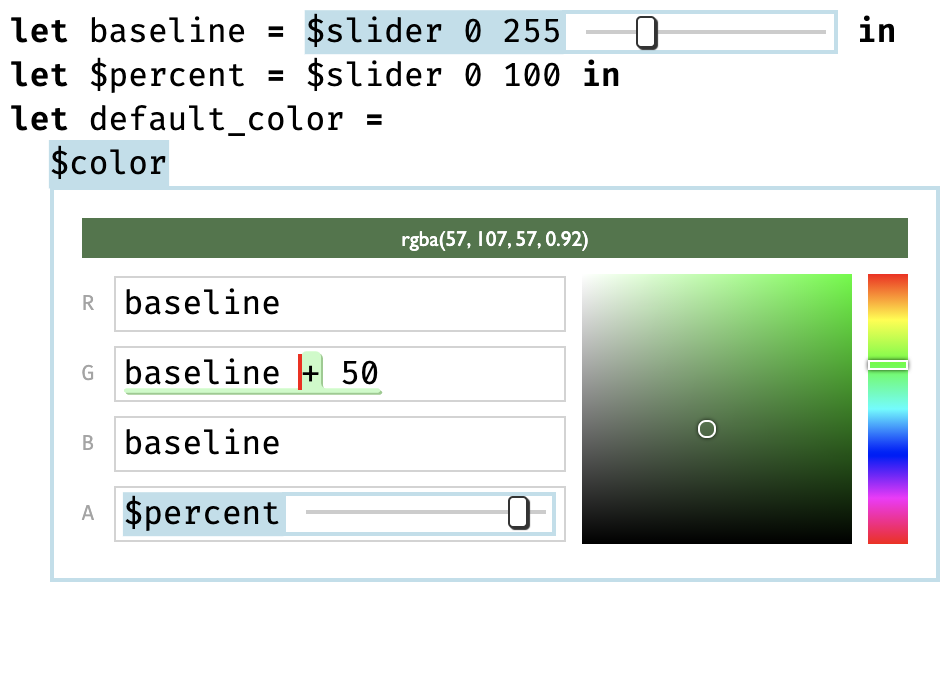
\includegraphics[width=\linewidth]{slider-color-livelits.png}
    \end{subfigure}
  \end{minipage}
  \hspace{3mm}
  \begin{subfigure}[t]{0.585\textwidth}
  \begin{snugshade}
   \vspace*{-2mm}
    \caption{\textbf{Case Study}: Grading with Livelits}
    \vspace*{1mm}
     \end{snugshade}
    \vspace*{1.5mm}
    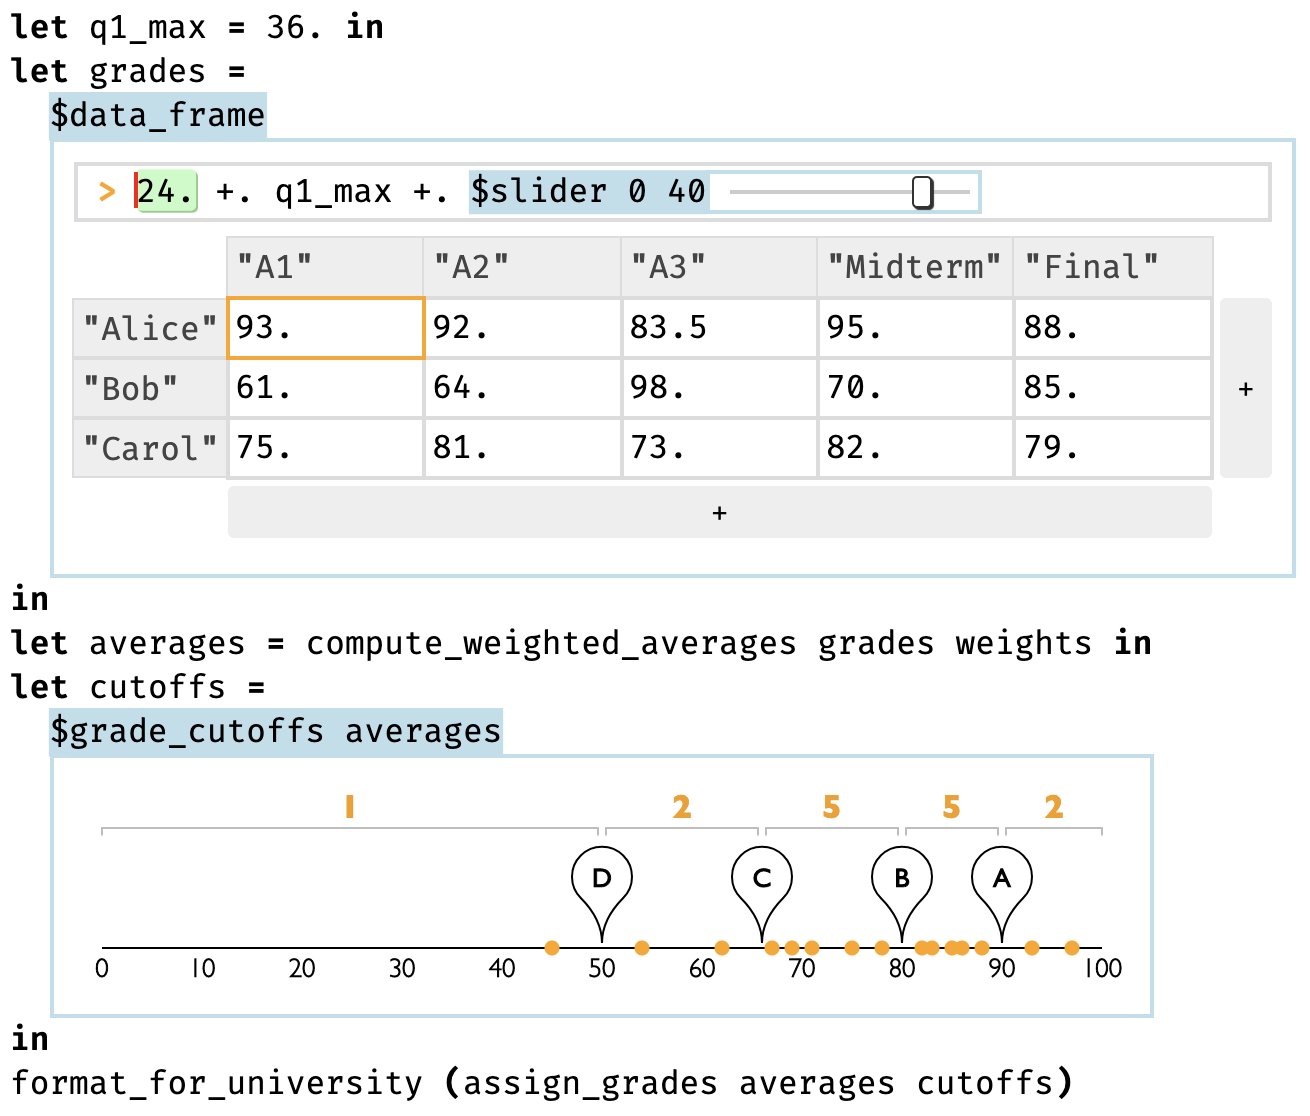
\includegraphics[width=\linewidth]{grade-cutoff-livelit.png}
  \end{subfigure}
   \caption{
   (a) This figure, adapted from the prior work of \citet{Graphite},
   shows a Graphite palette associated with the \texttt{Color} class.
   The client can specify the RGBA components only using literal numbers.
   (b) A similar Hazel livelit for colors uses live splices for the RGBA components,
   so the client can enter any Hazel expression.
   In this case, the client has entered a variable, itself defined using a slider livelit, into the RGB
   splices. The A splice is filled directly with a slider livelit.
   The color livelit evaluates splices under its closure to display the
   computed color.
   The value of \li{default\_color} is determined by the livelit via a macro expansion step.}
   \label{fig:color}
\end{figure*}

Of course, we are not the first to integrate direct manipulation interfaces
into symbolic programming environments.
% Prior work on projectional editing
% and active code completion, detailed in Sec. \ref{sec:related-work},
% has also considered the problem of entering expressions
% of certain types, like \li{Color},
% using specialized GUIs integrated into a program editor.
% We detail prior work in Sec.~\ref{sec:related-work}, but 
The prior work most relevant to this paper is the {Graphite} system for Eclipse for Java,
demonstrated in Fig.~\ref{fig:color}(a) \cite{Graphite}.
Graphite allows a library provider to associate a GUI, called a \emph{palette}, with a type 
(via a Java class annotation).
Wherever an expression of this type is needed,
i.e. wherever there is a \emph{hole} of that type in the program
(as determined by Eclipse's online parser and typechecker),
the environment offers the client the option, via the code completion menu,
to interact with the palette.
Once the interaction is finished, the palette generates a
Java expression to fill the hole.
Figure~\ref{fig:color}(a), adapted from this prior work, demonstrates a color palette invoked using Graphite.
When the user presses the \li{Enter} key, the Java expression \li{new Color(173, 173, 173, 85)} is inserted at the cursor and the palette disappears.
Several related systems, such as the  
\textbf{mage} system for the Jupyter notebook environment \cite{DBLP:conf/uist/KeryRHMWP20}
and the interactive visual syntax system for Racket \cite{interactive-visual-syntax}, behave fundamentally similarly.
asdfasdfa
fasdfasdf
asdfasd\todo{placeholder for future text that might be added}

\citet{Graphite} evaluated Graphite by surveying 473 developers 
and \citet{DBLP:conf/uist/KeryRHMWP20} evaluated \textbf{mage} by interviewing 9 developers.
Both studies found that
participants viewed the proposed mechanism favorably and 
would use a suitable GUI some or all of the time.
% \footnote{When presented with a color palette,
% many participants remarked that they rarely entered colors directly into Java code,
% but rather into stylesheets.
% Other palettes, e.g. a palette
% that supported regular expression construction, were viewed as more
% suitable for Java code.
% The mechanisms being considered are suitable both for general-purpose languages
% and typed domain-specific languages like typed stylesheets, which can often be embedded into modern
% general-purpose languages.}
This and other prior work also collectively showcase a wide variety of use cases \cite{Graphite,DBLP:conf/uist/KeryRHMWP20,interactive-visual-syntax}\todo{more cites}, 
and the Graphite survey solicited dozens of additional use cases from participants,
which the authors systematically taxonomize \cite{Graphite}. 
We take these extensive empirical findings   
as evidence for, and a showcase of, 
the value of this class of mechanisms for integrating GUIs into code.

\subsection{Contributions}

We turn our attention in this paper to several fundamental technical
deficiencies that limit GUI providers and clients using these prior systems.
To address these, 
we introduce a system of \emph{live literals}, or \emph{livelits}, 
demonstrated in Fig.~\ref{fig:color}(b). 
Livelits are unique in achieving all of the following properties.
(We describe which subset of these properties 
are achieved by prior systems,
including those just mentioned, 
in Sec.~\ref{sec:related-work}.)

\newcommand{\llproperty}[1]{\vspace{5px}\noindent\textbf{#1}.}

\llproperty{Decentralized Extensibility}
    Providers define livelits in libraries, and 
    clients invoke livelits by name. Livelit names, e.g. \li{\$color},  are prefixed by \li{\$},    
    to distinguish them from variables.
    % We call this \emph{decentralized extensibility}.
    % Both mage and Racket's visual syntax system are similarly extensible, 
    % but 
    % In Graphite, palettes are associated with class definitions, 
    % so there is a tighter association between 
    % Other systems, discussed in Sec.~\ref{sec:related-work}, 
    % are either non-extensible, or cannot be extended by library providers 
    % (only by, for example, separately installed editor extensions, or by 
    % regenerating the editor using a language workbench.)
 
\llproperty{Persistence}
  % In Graphite and \textbf{mage}, GUIs are {ephemeral},
  % i.e. they disappear after the initial interaction,
  % leaving behind only the generated textual code.
  % Only the programmer that initially enters the expression
  % benefits from the feedback and affordances that the GUI provides.
  % %
  % \footnote{Graphite does include an \emph{ad hoc} mechanism that
  % allows palettes to parse the code that is selected in the editor
  % when the palette loads, but this requires that each palette implement
  % a parser for the subset of Java used in the code that it generates,
  % and therefore this mechanism is quite brittle. It is also difficult
  % to persist GUI state that is not included in the generated code.}
  Livelits are persistent elements of the syntax tree. They operate as  
  graphical literals, rather than as the ephemeral code generation GUIs of Graphite and \textbf{mage}. 
  We define a pure model-view-update-expand architecture
  (a variation on Elm's model-view-update architecture \cite{ElmArchitecture}) 
  where only the model needs to be persisted.
  The dynamic meaning of a livelit is determined by macro expansion.
  % We chose the word ``literal'' rather than ``palette'' because,  persistence, livelits
  % operate as graphical literals.

\llproperty{Hygienic Composition}
% Prior systems have limited or no support for {entering sub-expressions within the GUI}, 
% so they are useful mainly for generating expressions composed of constants,
% e.g. color constants in Fig.~\ref{fig:color}(a).
%
  Livelits support sub-expressions directly in the GUI, which we call \emph{splices} (after
   \citet{TLMs}).
  Fig.~\ref{fig:color}(b) demonstrates splicing: the RGBA components  
  are splice editors, so the client can define a variable, \li{baseline},
  to relate the color components\todo{tweak figure}{} 
  and use a slider livelit inline to specify the alpha component.
  % Similarly, Fig.~\ref{fig:grading}(b)\todo{subfigure labels}{} demonstrates a 
  %  data table livelit where each entry is a splice.
  
  Crucially, composition is strictly 
  governed by a hygiene discipline that ensures
  (1) \textbf{capture avoidance}, i.e. that variables that the client uses in splices 
  will not capture expansion-internal bindings; and 
  (2) \textbf{context independence}, i.e. that the livelit 
  can be invoked in any program context.%without pre-condition or conflict.

\llproperty{Parameterization} Livelits can form parameterized families.
  For example, \li{\$slider} in Fig.~\ref{fig:color}(b) is parameterized by the slider's bounds.
  Parameters operate like splices, differing in that they can be partially applied in
  livelit abbreviations. For example, Fig.~\ref{fig:color}(b)\todo{add slider}{} 
  partially applies \li{\$slider} to \li{0} and \li{100} to define a \li{\$percentage} slider\todo{todo}{}.
  % \begin{lstlisting}[numbers=none]
  % let $percentage = $slider 0 100 in ...
  % \end{lstlisting}
  % Parameterization also underlies the hygiene mechanism, as we will discuss in Sec.~\ref{sec:livelit-definitions}.

\llproperty{Typing} Each livelit specifies the type of expansions it generates, 
and parameters and splices also specify types, 
so livelits are compatible with type-driven methodologies and tools.
Together with the hygiene discipline, this allow clients to reason abstractly about expansions, i.e.  
without inspecting the expansions or livelit implementations directly.

\llproperty{Liveness} Uniquely, livelits can evaluate splices 
  throughout the editing process 
  (i.e. in a \emph{live} manner \cite{DBLP:conf/icse/Tanimoto13}) 
  to provide feedback related to run-time behavior.
  For example, in Fig.~\ref{fig:color}(b), 
  displaying the selected color requires evaluating the RGBA
  component splices to numeric values.
  Evaluation occurs in a run-time environment (i.e. closure) determined by
  leaving the hole being filled by the livelit temporarily unfilled and then evaluating
  using a two-phased variant of the semantics for 
  live programming with typed holes developed by \citet{HazelnutLive}.
  We support live evaluation even for livelits 
  that appear inside a function. Multiple function calls lead 
  to multiple closures that the client 
   can select between.

\paragraph{Outline.} We begin in Sec.~\ref{sec:case-studies} by introducing
livelits from the perspective of client programmers. 
Our examples are organized into case studies 
and are chosen to demonstrate the novel contributions of this paper.
In Sec.~\ref{sec:livelit-definitions}, 
we consider the livelit provider's perspective by introducing livelit
definitions with a detailed example.
In Sec.~\ref{sec:livelit-calculus}, we define the \emph{typed livelit calculus}. 
We have mechanically specified the central mechanism, livelit expansion, and proven the associated metatheorems in Agda.
This calculus 
serves to capture the essential nature of livelits 
independent of the particularities of syntax, GUI frameworks, 
and other orthogonal design details,
because we believe livelits can be integrated into a wide variety of programming systems. 
In Sec.~\ref{sec:implementation}, we provide a more detailed account of our two implementations of livelits.
Our primary implementation, used in the screenshots in the paper,
is integrated into Hazel, a live programming environment designed 
around hole-driven development. 
We have also prototyped livelits within a standard text editor. 
Additionally, we discuss factors that must be considered when integrating livelits into languages with side effects.
In Sec.~\ref{sec:related-work}, we compare livelits to related work using the design properties outlined above 
as a rubric.
Finally, we conclude in Sec.~\ref{sec:discussion} after a discussion of present limitations and future work.